\documentclass[conference]{IEEEtran}
\IEEEoverridecommandlockouts
% The preceding line is only needed to identify funding in the first footnote. If that is unneeded, please comment it out.
\usepackage{cite}
\usepackage{amsmath,amssymb,amsfonts}
\usepackage{algorithmic}
\usepackage{graphicx}
\usepackage{textcomp}
\usepackage[colorlinks,bookmarksopen,bookmarksnumbered,citecolor=red,urlcolor=red]{hyperref}


\def\BibTeX{{\rm B\kern-.05em{\sc i\kern-.025em b}\kern-.08em
    T\kern-.1667em\lower.7ex\hbox{E}\kern-.125emX}}
\begin{document}

\title{Enabling Computational Literacy Through Center for Research Computing Resources}

\author{\IEEEauthorblockN{1\textsuperscript{st} Given Name Surname}
\IEEEauthorblockA{\textit{dept. name of organization (of Aff.)} \\
\textit{name of organization (of Aff.)}\\
City, Country \\
email address}
\and
\IEEEauthorblockN{2\textsuperscript{nd} Given Name Surname}
\IEEEauthorblockA{\textit{dept. name of organization (of Aff.)} \\
\textit{name of organization (of Aff.)}\\
City, Country \\
email address}
\and
\IEEEauthorblockN{3\textsuperscript{rd} Given Name Surname}
\IEEEauthorblockA{\textit{dept. name of organization (of Aff.)} \\
\textit{name of organization (of Aff.)}\\
City, Country \\
email address}
\and
\IEEEauthorblockN{4\textsuperscript{th} Given Name Surname}
\IEEEauthorblockA{\textit{dept. name of organization (of Aff.)} \\
\textit{name of organization (of Aff.)}\\
City, Country \\
email address}
\and
\IEEEauthorblockN{5\textsuperscript{th} Given Name Surname}
\IEEEauthorblockA{\textit{dept. name of organization (of Aff.)} \\
\textit{name of organization (of Aff.)}\\
City, Country \\
email address}
\and
\IEEEauthorblockN{6\textsuperscript{th} Given Name Surname}
\IEEEauthorblockA{\textit{dept. name of organization (of Aff.)} \\
\textit{name of organization (of Aff.)}\\
City, Country \\
email address}
}

\maketitle

\begin{abstract}
This document is a model and instructions for \LaTeX.
This and the IEEEtran.cls file define the components of your paper [title, text, heads, etc.]. *CRITICAL: Do Not Use Symbols, Special Characters, Footnotes, 
or Math in Paper Title or Abstract.
\end{abstract}

\begin{IEEEkeywords}
Storage systems, ZFS, HPC
\end{IEEEkeywords}



\section{Introduction}


The Center for Research Computing (CRC) is the University's closest thing to research computing.
While CRC maintains the University's largest cluster, the
funding model has resulted in a highly heterogeneous architecture that is essentially a {\it Frankenstein} of
many smaller clusters. In the past year, CRC tried to meet the following requirements:

\begin{itemize}

\item Merge any small portion of the cluster around the university. 

\item Significant investment in hardware, in terms of compute, storage and networking from the Provost Office had been made. 

\item The CRC grows in terms of personnel. Personnel are dedicated system administrators. These administrators are Ph.D. level scientists and are in charge of system admin, user admin and daily
technical support. They are also domain experts with high performance computing expertise with significant computational research experience. Research computing is the blending of traditional science with cutting-edge computational expertise. As such an excellent scientist with no computational skills will not
be successful in this space. Likewise, an excellent computer scientist/programmer will not be successful in this space. However, domain experts with both the science and computing background,
capable of interfacing with both traditional scientist and computer scientists are the glue required
for successful collaborations in research computing. Such a model is the status quo at all major
national labs and national computing centers.

\end{itemize}


The University of Pittsburgh is best served by servicing the missing middle. The missing middle is the void
between lab level and department level computing resources which order $O(10^1)-O(10^2)$ processors and national resources which order $O(10^5)-O(10^6)$ processors. In the same way that the
University's mission is to develop and prepare graduates for the workforce, research computing
at the University should develop and prepare computational researcher's for the utilization of
facilities at the largest scale (national labs).

\begin{itemize}
\item Outreach
\item Training (example is Barmeda's workshop, Bio-Stat course for undergraduate students.
\item Workforce developement
\item Hacketown
\end{itemize}



\begin{figure}
    \centering
    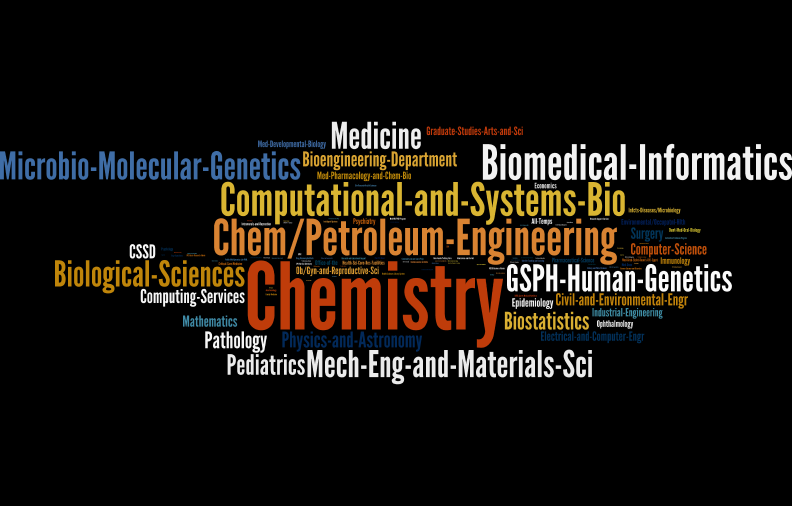
\includegraphics[width=3in]{wordle1}
    \caption{The wordle of number of users on CRC computational resources.}
    \label{fig:wordle1}
\end{figure}


\section{CRC resources}
The cluster compute nodes were purchased with funds provided by the University, by faculty researchers, and by a NSF Major Research Instrumentation grant. Connectivity between the cluster and main campus is via two 100Gbps fibers and to Internet2 via 100Gbps.  The cluster is comprised of: 104 nodes of 24-core Skylake, 96 nodes of 28-core Intel Xeon Broadwell, 20 nodes of 16-core Intel Xeno Haswell-EP, 32 nodes of 20-core Intel Xeon Haswell, 53 nodes of 12-core Xeon Broadwel, and 8 nodes of 256-core knights landing (KNL). The nodes
have a range of 12GB to 512GB per node shared memory. Twenty four of the 12-core nodes have a total of 32 general
purpose GTX1080, 28-Titan X, and 2-K40 GPU accelerator cards in order to support hybrid parallelization efforts. Furthermore, a dedicated node comprised of 28-cores Intel Xeon Broadwell CPUs and 2-GTX1080 GPU card is built to support the visualization effort around the campus.
The nodes
are clustered via a fast Intel Omni-Path (OPA) or Infiniband low latency network fabrics in order to enable efficient distributed parallel
(MPI based) runs. The global storage is comprised of a 130TB Isilon home space (which is backed up), 80 TB of standard NFS home space, a 450 TB Lustre parallel filesystem, and 1PB ZFS filesystem for archival. This infrastructure is designed for future scaling via additional resources funded by research instrumentation grants, internal University funds, or faculty contributions from grants or start-up funds. The cluster operating systems are Redhat Enterprise Linux 6 and 7. A very wide range of major software packages are licensed and installed on the cluster, ranging from quantum mechanics (e.g., Gaussian, Molpro, VASP, CP2K, QMC), to classical mechanics (e.g., NAMD, LAMMPS, Amber), to continuum mechanics (e.g., Abaqus, ANSYS, COMSOL, Lumerical), to genomics analysis suits (e.g., Tophat/Bowtie, CLCb Genomics Server).

\subsection{Computational modeling \& simulation program}
The computational modeling \& simulation program at the university of Pittsburgh offer its graduate students with an integrated program of creative, independent research, course work, and teaching. Students in this program get heavy doeses of graduate applied mathematics/statistics, computer science and high performance computing using CRC resources. During the past academic year, the center hired one of the CMS Ph.D. graduates as a HPC consultants.  


\subsection{Seminars}

\subsection{Workshops}

CRC offers numerous workshops targeting undergraduate and graduate students from all majors. 

\subsection*{Cluster usage training}

\subsection*{Hybrid OpenMP/MPI programming}
This workshop consists of three days workshops on OpenMP, MPI, and Hybrid OpenMP/MPI parallelism. The course was designed to 

\begin{itemize}
\item Emerging trends in high-performance computing hardware
\item Technical reasons for trending towards multicore
\item Processor architectures are inherently parallel in design
\item What does shared memory mean from a hardware perspective?
\item What does distributed memory mean from a hardware perspective?
\item How about  a hybrid of shared and distributed memory system?
\item Programming models and why go hybrid MPI-X?
\item Simple programming problems for thought
\end{itemize}


\subsection*{R programming}
\subsection*{Python programming through JupyterHub}

\subsection*{C/C++ programming}
The workshop covers:
    \begin{itemize}
    \item Variables, Constants, and Containers
    \item Flow Control
    \item Loops
    \item Functions
    \item Structures
    \item File I/O
    \item Compilation
    \item Vectorization
    \end{itemize}

\subsection*{Basic Linux}
\subsection*{Intel compiler tools}
\subsection*{Advanced Linux}
\subsection*{CUDA programming}
\subsection*{Genomics pipeline}


\subsection{Courses}
In  addition  to  the  workshops that provide  resources, we engage in the development of computational courses which counts as the program requirements for student. These courses and the projects included in their syllabus are  growing  need  in  extra  curricular  activities
and applied courses. Integrating HPC into these project-based
activities  is  crucial  in  order  to  introduce  students  to  HPC  in
a setting that allows for exploration. These set of activities encourage student to learn about computational tools and help them toward their career' decision making. Here are the courses offered with collaboration with CRC:

\subsection*{Computational Biology}
for undergraduate student in XXX semester



\begin{table}[]
\centering
    \begin{tabular}{c|c}

      Semester   & Courses \\
      \hline
        Fall 2013 & 4 \\
        Spring 2014 & 4 \\
        Fall 2014 & 4 \\
        Spring 2015 & 4 \\
        Fall 2015 & 4 \\
        Spring 2016 & 4 \\
        Fall 2017 & 5 \\
        Spring 2018 & 6 
    \end{tabular}
    \label{tab:my_label}
    \caption{Courses using CRC resources per semester.}
\end{table}

\subsection*{Data Science}

\subsection*{Computational Physics}
.
.
.


\subsection{Engagement}
One of the main duties of Consultants at CRC is meeting with	researchers	in order to better	understand their computational needs and to help them select appropriate resources and approaches. These engagements are important for accelerating the adoption of ACI resources in support of research endeavors. At Pitt, we are also engaged in face-to-face meeting with researchers. For that, regular office hours are assigned so that students can meet with CRC team.

\subsection{Effort to be done}
Compute is
cheap, storage is not, having all storage backed up is even more expensive. The University needs
to recognize that this requires significant investment, especially in regards to big data. Moreover,
an upgrade path and budget to replace and extend these resources needs to be in place.


\section{Lessons Learned}

\subsection*{Outreach}
Advanced computing can benefit many research areas that have not traditionally been routine users of computing beyond the laptop.  While many researchers are vaguely aware of such possibilities, they often do not appreciate the accessibility to powerful computing resources that they have here at Pitt, and perhaps even more importantly, the accessibility they have to expert advice on how to exploit such computing power. A major opportunity for the newly formed Center for Research Computing is to reach out to such researchers and engage them in exploring how we can improve their research productivity through the use of advanced computing.

We have already made significant strides in this effort, including beginning discussions with faculty in economics, nursing, digital humanities, information science, biology, human genetics, public health, biomedical informatics, computer science, statistics, emergency medicine, and the health system library.

We also presented an all-day Symposium on Urban Computing and Machine Learning, which had two plenary speakers, nine invited talks, 24 posters, and around 100 attendees. Advanced Research Computing Symposium is a semi-annual meeting organized by the University of Pittsburgh's CRC. The symposium will consist of invited lectures that cover data intensive computing in astrophysics and computational biophysics aimed at a general audience including scientists and engineers.




\subsection*{Undergraduate students participation}
In FY17, we supported 330 Pitt faculty and students in their research endeavor from 37 departments. This includes 52 undergraduate users and 132 graduate students. We mentored 2 undergraduates as part of the First Experience in Research program (one continued as a mentee in an independent study course). We also organized an undergraduate course in Bio-Statistics. We expect that we have the balanced participation between graduate toward undergraduate in near future.  


\section{Conclusion}

The CRC resources has been proven to be very effective tool for workshops and courses for the Pitt community. The number of courses has been growing for over past few years. We also would like to build a dedicated cluster for teaching purposes. Integration of computational courses from all the different fields with CRC cyberinfrastructure is a key advantage of the CRC.

CRC's workshops and courses in general research computing and field specific topics continue to expand in order to address the computational needs and techniques used by our users. Theses workshops and courses targeted students and researchers and learn theoretical concepts through extensive hands-on exercises.  

For the future, we will focus on continuing our general workshops and design the hands-on based on the students and researchers' demand. We also would like to cover some of the data-intensive programming tools such as Spark, Hadoop and Machine Learning analysis. 


%ACKNOWLEDGMENTS are optional
\section{Acknowledgments}
Acknowledge CRC.
%
% The following two commands are all you need in the
% initial runs of your .tex file to
\bibliographystyle{abbrv}
\bibliography{ref} 
\end{document}

====== IGNORE ========
Comments and brainstorming go here!

High Performance Computing (HPC) and, in general, Parallel and Distributed Computing (PDC) has become pervasive, from supercomputers and server farms containing multicore CPUs and GPUs, to individual PCs, laptops, and mobile devices. Even casual users of computers now depend on parallel processing. Therefore it is important for every computer user (and especially every programmer) to understand how parallelism and distributed computing affect problem solving. It is essential for educators to impart a range of PDC and HPC knowledge and skills at multiple levels within the educational fabric woven by Computer Science (CS), Computer Engineering (CE), and related computational curricula including data science. Companies and laboratories need people with these skills, and, as a result, they are finding that they must now engage in extensive on-the-job training. Nevertheless, rapid changes in hardware platforms, languages, and programming environments increasingly challenge educators to decide what to teach and how to teach it, in order to prepare students for careers that are increasingly likely to involve PDC and HPC.

This workshop invites unpublished manuscripts from academia, industry, and government laboratories on topics pertaining to the needs and approaches for augmenting undergraduate and graduate education in Computer Science and Engineering, Computational Science, and computational courses for both STEM and business disciplines with PDC and HPC concepts.  We also encourage papers on large-scale data science.

The workshop is particularly dedicated to bringing together stakeholders from industry (both hardware vendors and employers), government labs, and academia in the context of SC-17.  The goal is for each to hear the challenges faced by others, to learn about various approaches to addressing these challenges, and to have opportunities to exchange ideas and solutions. In addition to contributed talks, this workshop may feature invited talks on opportunities for collaboration, resource sharing, educator training, internships, and other means of increasing cross-fertilization between industry, government, and academia.

Topics of interest include, but are not limited to:

1. Pedagogical issues in incorporating PDC and HPC in undergraduate and graduate education, especially in core courses
2. Novel ways of teaching PDC and HPC topics
3. Data Science and Big Data aspects of teaching HPC/PDC including early experience with data science degree programs.
4. Experience with incorporating PDC and HPC topics into core CS/CE courses and in domain Computational Science and Engineering courses
5. Pedagogical tools, programming environments, infrastructures, languages, and projects for PDC and HPC
6. Employers' experiences with and expectation of the level of PDC and HPC proficiency among new graduates
7. Education resources based on higher-level programming languages, models, and environments such as PGAS, X10, Chapel, Haskell, Python, Cilk, CUDA, OpenCL, OpenACC, and Hadoop  
8. Parallel and distributed models of programming and computation suitable for teaching, learning, and workforce development.
9. Projects or units that introduce students to concepts relevant to Internet of Things, networking, or other topics in mobile devices or sensor networks.
10. Issues and experiences addressing the gender gap in computing and broadening participation of underrepresented groups.
